\documentclass[12pt, a4paper]{article}
\usepackage[headheight=18pt, top=25mm, bottom=25mm, left=25mm, right=25mm]{geometry}
\usepackage[polish]{babel}
\usepackage[utf8]{inputenc}
\usepackage[T1]{fontenc}
\frenchspacing
\usepackage{comment}
\usepackage{hyperref}
\usepackage{graphicx}
\usepackage{amsmath}
\usepackage{hanging}
\usepackage{longtable}
\usepackage{listings}
\usepackage{float}
\usepackage{refcount}                   % Refers to another footnote
\usepackage[hang,flushmargin]{footmisc} % Removes indentation in footnote
\usepackage{caption}                    % Caption width
\usepackage{fixltx2e}                   % Subscript for text mode
\lstset{basicstyle=\tt,breaklines=true}

\hypersetup{
    colorlinks  =   true,                   
    linkcolor   =   black,                  
    citecolor   =   black,                  
    urlcolor    =   blue                    
}
\urlstyle{same}

\title{Zaawansowane techniki analizy danych \\\Large Zadanie projektowe}
\author{Krzysztof Radosław Osada}
\date{\today}

\begin{document}
\maketitle

\section*{Ćwiczenie nr 1}

\begin{hangparas}{2.025cm}{1}
  \textbf{Problem:} Znaleźć odpowiednie do analizy dane, w których można wyróżnić co najmniej 3 populacje.\newline
\end{hangparas}

\begin{hangparas}{2.9cm}{1}
\textbf{Rozwiązanie:} Danymi poddanymi analizie będą tabele kursów średnich walut obcych z~dni 17\footnote{\noindent Narodowy Bank Polski. \textit{Tabela nr 244/A/NBP/2018 z dnia 2018-12-17}.\\\url{https://www.nbp.pl/home.aspx?navid=archa&c=/ascx/tabarch.ascx&n=a244z181217}\\Dostępny: 15.01.2019.}, 24\footnote{\noindent Narodowy Bank Polski. \textit{Tabela nr 249/A/NBP/2018 z dnia 2018-12-24}.\\\url{https://www.nbp.pl/home.aspx?navid=archa&c=/ascx/tabarch.ascx&n=a249z181224}\\Dostępny: 15.01.2019.} i 31\footnote{\noindent Narodowy Bank Polski. \textit{Tabela nr 252/A/NBP/2018 z dnia 2018-12-31}.\\\url{https://www.nbp.pl/home.aspx?navid=archa&c=/ascx/tabarch.ascx&n=a252z181231}\\Dostępny: 15.01.2019.} grudnia 2018 roku, przygotowane przez Narodowy Bank Polski. Zakładamy, że jedna populacja zawiera wartości wszystkich kursów średnich z~danego dnia, stąd zbiór danych jest złożony z próbek z 3 populacji.
\newline Dane po przetworzeniu zostały zapisane do pliku \texttt{kursy\_walut.csv} i zaprezentowane w Tabeli \ref{table:nbp} niniejszego dokumentu.
\end{hangparas}

\begin{longtable}{|l|l|l|l|}\hline
  \multicolumn{1}{|c}{\bf Nazwa waluty} & \multicolumn{1}{|c}{\bf 17 XII} & \multicolumn{1}{|c}{\bf 24 XII} & \multicolumn{1}{|c|}{\bf 31 XII} \\\hline
  bat                     & 0.1155 & 0.1154 & 0.1161 \\\hline 
  dolar amerykański       & 3.7871 & 3.7588 & 3.7597 \\\hline 
  dolar australijski      & 2.7194 & 2.6535 & 2.6549 \\\hline 
  dolar Hongkongu         & 0.4847 & 0.4800 & 0.4801 \\\hline 
  dolar kanadyjski        & 2.8309 & 2.7684 & 2.7620 \\\hline 
  dolar nowozelandzki     & 2.5804 & 2.5319 & 2.5230 \\\hline 
  dolar singapurski       & 2.7549 & 2.7367 & 2.7599 \\\hline 
  euro                    & 4.2906 & 4.2832 & 4.3000 \\\hline 
  forint                  & 1.3265 & 1.3315 & 1.3394 \\\hline 
  frank szwajcarski       & 3.8025 & 3.7777 & 3.8166 \\\hline 
  funt szterling          & 4.7718 & 4.7544 & 4.7895 \\\hline 
  hrywna                  & 0.1358 & 0.1373 & 0.1357 \\\hline 
  jen                     & 3.3413 & 3.3839 & 3.4124 \\\hline 
  korona czeska           & 0.1663 & 0.1655 & 0.1673 \\\hline 
  korona duńska           & 0.5747 & 0.5736 & 0.5759 \\\hline 
  korona islandzka        & 3.0779 & 3.2156 & 3.2282 \\\hline 
  korona norweska         & 0.4393 & 0.4290 & 0.4325 \\\hline
  korona szwedzka         & 0.4172 & 0.4143 & 0.4201 \\\hline
  kuna                    & 0.5802 & 0.5770 & 0.5799 \\\hline 
  lej rumuński            & 0.9217 & 0.9230 & 0.9229 \\\hline 
  lew                     & 2.1938 & 2.1900 & 2.1985 \\\hline 
  lira turecka            & 0.7042 & 0.7081 & 0.7108 \\\hline 
  nowy izraelski szekel   & 1.0030 & 0.9949 & 1.0008 \\\hline
  peso chilijskie         & 0.5539 & 0.5420 & 0.5417 \\\hline 
  peso filipinskie        & 0.0715 & 0.0709 & 0.0716 \\\hline 
  peso meksykańskie       & 0.1881 & 0.1890 & 0.1915 \\\hline 
  rand                    & 0.2646 & 0.2581 & 0.2614 \\\hline 
  real                    & 0.9668 & 0.9628 & 0.9687 \\\hline 
  ringgit                 & 0.9058 & 0.8983 & 0.9098 \\\hline 
  rubel rosyjski          & 0.0570 & 0.0549 & 0.0541 \\\hline 
  rupia indonezyjska      & 2.5984 & 2.5825 & 2.6146 \\\hline 
  rupia indyjska          & 5.2872 & 5.3715 & 5.3875 \\\hline 
  won poludniowokoreański & 0.3348 & 0.3342 & 0.3373 \\\hline 
  yuan renminbi           & 0.5490 & 0.5448 & 0.5481 \\\hline
  \caption{kursy średnie walut obcych w XII 2018 r.}
  \label{table:nbp}
\end{longtable}

\section*{Ćwiczenie nr 2}

\begin{hangparas}{2.1cm}{1}
  \textbf{Problem:} Określić parametry rozkładu poszczególnych populacji: średnią, odchylenie standardowe, minimum, maksimum, mediana, pierwszy kwartyl i trzeci kwartyl.\newline
\end{hangparas}

\begin{hangparas}{2.85cm}{1}
\textbf{Rozwiązanie:} Skorzystać z wbudowanych funkcji Matlaba w celu wyznaczenia wymienionych parametrów (zob. Listing \ref{listing:c2}).\newline
\end{hangparas}
\begin{lstlisting}[frame=single,label={listing:c2},caption={fragment rozwiązania ćwiczenia nr 2.},captionpos=b]
M = csvread('kursy_walut.csv', 1, 1)
mean_               = mean(M)
standard_deviation  = std(M)
minimum             = min(M)
maximum             = max(M)
median_             = median(M)
first_quartile      = quantile(M, 0.25)
\end{lstlisting}

Warto zauważyć, że czytanie danych przy użyciu funkcji \texttt{csvread} powinniśmy rozpocząć od drugiego wiersza i drugiej kolumny, tak by opuścić tytuły kolumn i nazwy walut, które nie są istotne w naszej analizie.\newline

\noindent Uzyskane wyniki zostały przedstawione w Tabeli \ref{table:c2}.

\begin{longtable}{|l|l|l|l|}\hline
  \multicolumn{1}{|c}{\bf Parametr} & \multicolumn{1}{|c}{\bf P1\footnote{\label{note:P}Ilekroć mowa o ,,P1'', ,,P2'' lub ,,P3'', to są to odpowiednio populacje pierwsza, druga lub trzecia.}} & \multicolumn{1}{|c}{\bf P2\footnotemark[\getrefnumber{note:P}]} & \multicolumn{1}{|c|}{\bf P3\footnotemark[\getrefnumber{note:P}]}\\\hline
  średnia                 & 1.6117 & 1.6092 & 1.6168\\\hline
  odchylenie standardowe  & 1.5522 & 1.5569 & 1.5641\\\hline
  minimum                 & 0.0570 & 0.0549 & 0.0541\\\hline
  maksimum                & 5.2872 & 5.3715 & 5.3875\\\hline
  mediana                 & 0.9138 & 0.9106 & 0.9163\\\hline
  pierwszy kwartyl        & 0.4172 & 0.4143 & 0.4201\\\hline
  trzeci kwartyl          & 2.7549 & 2.7367 & 2.7599\\\hline
  \caption{podstawowe parametry badanych próbek z populacji.}
  \label{table:c2}
\end{longtable}

\section*{Ćwiczenie nr 3}
\begin{hangparas}{2cm}{1}
  \textbf{Problem:} Sprawdzić równość badanej cechy we wszystkich populacjach przy użyciu odpowiedniego testu. Pamiętać o zweryfikowaniu, czy: zmienne są powiązane, wariancje są równe i z jakiego rozkładu pochodzą dane; w razie potzeby wykonać analizę post-hoc.\newline
\end{hangparas}

\begin{hangparas}{2.85cm}{1}
\textbf{Rozwiązanie:} Na samym początku musimy sprawdzić, czy próbki z populacji pochodzą z rozkładu normalnego. Każda próbka jest stosunkowo niewielka (zawiera 33 elementy), stąd możemy wysunąć odpowiednie hipotezy i skorzystać z testu \textbf{Shapiro-Wilka.}\newline
\end{hangparas}

\textbf{H0\textsubscript{(1)}:} P1 pochodzi z rozkładu normalnego. \newline
\textbf{H1\textsubscript{(1)}:} P1 nie pochodzi z rozkładu normalnego. \newline
\textbf{H0\textsubscript{(2)}:} P2 pochodzi z rozkładu normalnego. \newline
\textbf{H1\textsubscript{(2)}:} P2 nie pochodzi z rozkładu normalnego. \newline
\textbf{H0\textsubscript{(3)}:} P3 pochodzi z rozkładu normalnego. \newline
\textbf{H1\textsubscript{(3)}:} P3 nie pochodzi z rozkładu normalnego. \newline

\begin{lstlisting}[frame=single,label={listing:c31},caption={badanie, czy próbki pochodzą z rozkładu normalnego.},captionpos=b]
M  = csvread('kursy_walut.csv', 1, 1)
C1 = M(:, 1) 
C2 = M(:, 2) 
C3 = M(:, 3)
[swh1, swp1, swstats1] = swtest(C1)
[swh2, swp2, swstats2] = swtest(C2)
[swh3, swp3, swstats3] = swtest(C3)
\end{lstlisting}

Otrzymane wyniki (zob. Tabela \ref{table:c31}) skłaniają do odrzucenia \textbf{wszystkich} hipotez zerowych na korzyść hipotez alternatywnych. Przyjmujemy więc, że żadna z próbek nie pochodzi z rozkładu normalnego (por. Rysunki \ref{fig:c61}, \ref{fig:c62} i \ref{fig:c63}).

W tej sytuacji możemy korzystać tylko z testów, które nie wymagają spełnienia założenia normalności rozkładu. \textbf{Test U Manna-Whitneya} pozwoli nam na zweryfikowanie tego, czy dla każdej pary populacji zmienne z próbki A są większe od zmiennych z próbki B tak często, jak zmienne z próbki B są większe od zmiennych z próbki B.

\begin{center}
  \begin{tabular}{|c|c|c|}\hline
    \tt swh1 & \tt swh2 & \tt shw3 \\\hline
    1 & 1 & 1 \\\hline
  \end{tabular}
  \captionof{table}{wartości uzyskane po wykonaniu kodu z Listingu \ref{listing:c31}.}
  \label{table:c31}
\end{center}

\noindent Zdefiniujmy więc nowe hipotezy:\newline

\noindent
\textbf{H0\textsubscript{(12)}:} wartości próbek z P1 i P2 są jednakowo duże. \newline
\textbf{H1\textsubscript{(12)}:} wartości próbek z P2 i P2 nie są jednakowo duże. \newline
\textbf{H0\textsubscript{(23)}:} wartości próbek z P2 i P3 są jednakowo duże. \newline
\textbf{H1\textsubscript{(23)}:} wartości próbek z P2 i P3 nie są jednakowo duże. \newline
\textbf{H0\textsubscript{(13)}:} wartości próbek z P1 i P3 są jednakowo duże. \newline
\textbf{H1\textsubscript{(13)}:} wartości próbek z P1 i P3 nie są jednakowo duże. \newline

\begin{lstlisting}[frame=single,label={listing:c32},caption={badanie, czy wartości próbek z populacji są jednakowo duże.},captionpos=b]
stats_12 = mwwtest(C1, C2)
stats_23 = mwwtest(C2, C3)
stats_13 = mwwtest(C1, C3)
\end{lstlisting}

Po wywołaniu funkcji \texttt{mwwtest} jak na Listingu \ref{listing:c32} otrzymamy pary wartości parametru $p$: \texttt{1-tailed} (dla hipotezy jednostronnej) i \texttt{2-tailed} (dla hipotezy dwustronnej); dla zadanych hipotez alternatywnych H1\textsubscript{(12)}, H1\textsubscript{(13)} i H1\textsubscript{(23)} będą nas interesować wartości parametru $p$ oznaczone jako \texttt{2-tailed}.

\begin{center}
  \begin{tabular}{|c|c|c|}\hline
    \tt stats\_12.p(2) & \tt stats\_23.p(2) & \tt stats\_13.p(2) \\\hline
    0.9755 & 0.8975 & 0.8975 \\\hline
  \end{tabular}
  \captionof{table}{wartości uzyskane po wykonaniu kodu z Listingu \ref{listing:c32}.}
  \label{table:c32}
\end{center}

Ponieważ uzyskane wyniki parametru $p$ dla wszystkich badanych par próbek z populacji (P1 i P2, P2 i P3 oraz P1 i P3) są znacząco większe od zakładanego poziomu istotności (0.05), \textbf{nie mamy podstaw do odrzucenia hipotez zerowych} głoszących, że próbki z~populacji są jednakowo duże. Innymi słowy, przyjmujemy, że kursy średnie walut obcych były takie same w kolejnych dniach (17, 24 i 31 grudnia).

\section*{Ćwiczenie nr 4}
\textit{To be continued...}

\section*{Ćwiczenie nr 5}

\section*{Ćwiczenie nr 6}
\begin{hangparas}{2.1cm}{1}
  \textbf{Problem:} Wyznaczyć (jeśli to możliwe) 95\% i 99\% przedział ufności dla średniej oraz wariancji dla każdej populacji.\newline
\end{hangparas}

\begin{hangparas}{2.85cm}{1}
\textbf{Rozwiązanie:} Wyznaczenie oczekiwanych parametrów \textbf{nie jest} możliwe -- żadna z próbek z populacji nie pochodzi z rozkładu normalnego.\newline
\end{hangparas}

\begin{figure}[H]
\centering
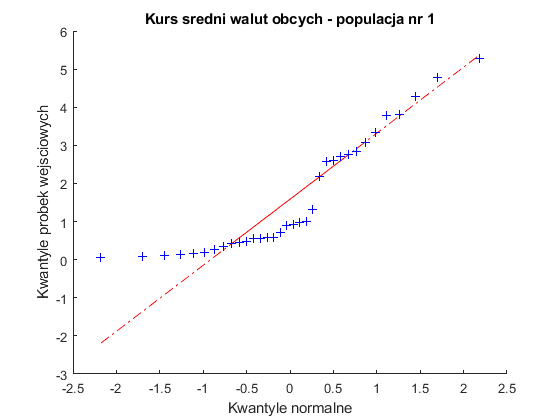
\includegraphics[width=.75\textwidth]{qqplot1.png}
\caption{Wykres Q--Q dla populacji nr 1.}
\label{fig:c61}
\end{figure}

\begin{figure}[H]
\centering
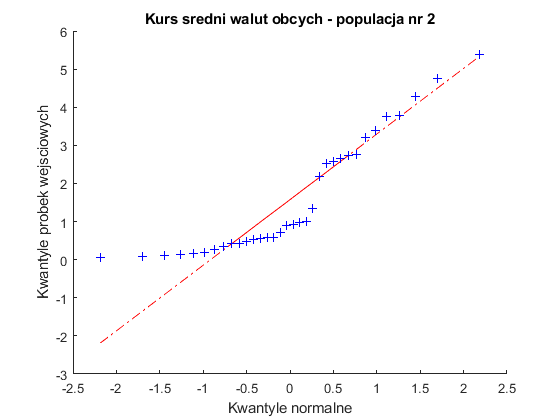
\includegraphics[width=.75\textwidth]{qqplot2.png}
\caption{Wykres Q--Q dla populacji nr 2.}
\label{fig:c62}
\end{figure}

\begin{figure}[H]
\centering
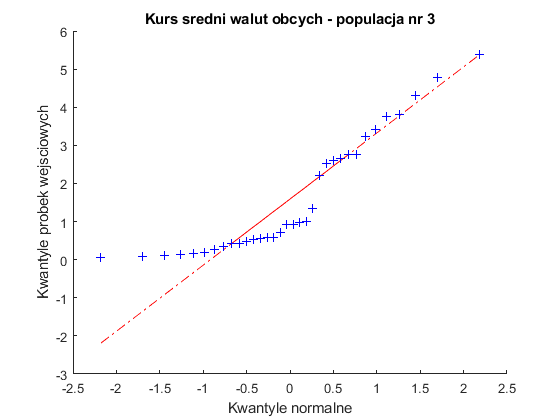
\includegraphics[width=.75\textwidth]{qqplot3.png}
\caption{Wykres Q--Q dla populacji nr 3.}
\label{fig:c63}
\end{figure}

\end{document}